\documentclass[11pt,a4paper]{article}
\usepackage[T1]{fontenc}
\usepackage[english]{babel}
\usepackage[latin1]{inputenc}
\usepackage{graphicx}
\usepackage{amsmath,amssymb}
\usepackage{siunitx}
	\sisetup{exponent-product = \cdot}
 	\sisetup{separate-uncertainty = true}
\usepackage{booktabs}
\usepackage[font=small,labelfont=bf]{caption}
\usepackage{enumitem}

\usepackage[scr]{rsfso}
\newcommand{\Laplace}{\mathcal{L}}

\begin{document}

\title{TMA4120 - Assignment 1} 
\author{William Dugan}

\maketitle

\section*{6.1.1}
\begin{align*}
	f(t) &= 2t + 8 \\
	\Laplace\{f\}(s) &= 2 \cdot \Laplace\{t\}(s) + 8 \cdot \Laplace\{1\}(s) 
		\hspace*{1cm} \text{ (Linearity)} \\
	&= \frac{2}{s^2} + \frac{8}{s} \\
	&= \frac{8s + 2}{s^2}
\end{align*}

\section*{6.1.12}
From the graph we can obtain the following equation for $f$;
\begin{align*}
	f(t) = 
	\left\{\begin{matrix}
	t & 0 \leq t < 1 \\ 
	1 & 1 < t < 2 \\ 
	0 & t \ge 2.
	\end{matrix}\right.
\end{align*}
\begin{align*}
	\Laplace\{f\}(s) 
	&= \Laplace\{t [u(t) - u(t-1)]\} + \Laplace\{u(t-1) - u(t-2)\} \\
	&= \Laplace\{tu(t)\} - \Laplace\{tu(t-1)\} + \Laplace\{u(t-1)\} - \Laplace\{u(t-2)\} \\
	&= \frac{1}{s^2} - \Laplace\{[(t-1)+1]u(t-1)\} + \frac{e^{-s}}{s} - \frac{e^{-2s}}{s} \\
	&= \frac{1}{s^2} - \frac{e^{-s}}{s} - \frac{e^{-s}}{s^2} + \frac{e^{-s}}{s} - \frac{e^{-2s}}{s} \\
	&= \frac{1}{s^2} - \frac{e^{-s}}{s^2} - \frac{e^{-2s}}{s}
\end{align*}

\section*{6.1.23}
Given $\Laplace\{f(t)\}(s) = F(s)$ and a positive constant $c > 0$, we have
\begin{align*}
	\Laplace\{f(ct)\}(s)
	&= \int_0^{\infty} e^{-st}f(ct)dt \\
	&= \frac{1}{c} \int_0^{\infty} e^{-sx/c}f(x)dx, \hspace*{.5cm} x=ct,\ dt = dx/c\\
	&= \frac{1}{c} F(s/c)
\end{align*}
Using $\Laplace\{\cos bt\}(s) = \frac{s}{s^2 + b}$ we get
\begin{align*}
	\Laplace\{\cos\omega t\}(s) 
	&= \frac{1}{\omega} \frac{s/\omega}{(s/\omega)^2 + 1} \\
	&= \frac{s}{s^2 + \omega^2}
\end{align*}

\section*{6.1.26}
\begin{align*}
	F(s) 
	&= \frac{5s+1}{s^2-25}
	= \frac{5s+1}{(s+5)(s-5)} 
	= \frac{A}{s+5} + \frac{B}{s-5}
	\rightarrow \frac{12}{5(s+5)} + \frac{13}{5(s-5)} \\
	\Laplace^{-1}\{F(s)\}(t) 
	&= \Laplace^{-1}\left\{\frac{12}{5(s+5)}\right\} + \Laplace^{-1}\left\{\frac{13}{5(s-5)}\right\} \\
	&= \frac{12}{5} e^{-5t} + \frac{13}{5} e^{5t} \\
	&= \frac{1}{5} (12e^{-5t} + 13e^{5t})
\end{align*}

\section*{6.1.36}
\begin{align*}
	f(t) 
	&= \sinh t \cos t \\
	&= \frac{1}{2} (e^t - e^{-t}) \cos t \\
	&= \frac{1}{2} e^t \cos t - \frac{1}{2} e^{-t} \cos t \\
	\Laplace\{f\}
	&= \frac{1}{2} \Laplace\{e^t\cos t\} - \frac{1}{2} \Laplace\{e^{-t}\cos t\} \\
	&= \frac{1}{2} [F(s-1) - F(s+1)] \\
	&= \frac{1}{2} \left[
		\frac{s-1}{(s-1)^2 + 1} - \frac{s+1}{(s+1)^2 + 1}
	\right]
\end{align*}

\section*{6.1.40}
\begin{align*}
	F(s)
	&= \frac{4}{s^2 - 2s - 3}
	= \frac{4}{(s-3)(s+1)}
	= \frac{A}{s-3} + \frac{B}{s+1}
	\rightarrow \frac{1}{s-3} - \frac{1}{s+1} \\
	\Laplace^{-1}\{F\}
	&= \Laplace^{-1}\left\{\frac{1}{s-3}\right\} - \Laplace^{-1}\left\{\frac{1}{s+1}\right\}
	= e^{3t} - e^{-t}
\end{align*}

\section*{6.2.4}
I wrote down the wrong values from the book so I will be solving the IVP $y'' + \underline{y'} = 10e^{-t}$ with $y(0) = 0 = y'(0)$. \\
\begin{itemize}[leftmargin=4.0cm,labelsep=0.5cm]
\item[$\Laplace$ - transform:]
	$\Laplace\{y''+y'\} = \Laplace\{10e^{-t}\}
	\rightarrow s^2 Y + sY = \frac{10}{s+1}$
\item[Solve for $Y$:]
	$Y = \frac{10}{s(s+1)^2}
	= \frac{A}{s} + \frac{B}{s+1} + \frac{C}{(s+1)^2}$
\item[Write as partial fraction:]
	$(A+C)s^2 + (A+B+2C)s + C = 10 \\
	\rightarrow A=-10,\ B=-10,\ C = 10 \\
	\rightarrow Y = \frac{10}{s} - \frac{10}{s+1} - \frac{10}{(s+1)^2}$
\item[Inverse $\Laplace$ -transform:]
	$ y = \Laplace^{-1}\{Y\} = -10e^{-t} - 10te^{-t} + 10$ (from table.)
\item[Control:]
	$ y(0) = -10 - 0 + 10 = 0 \\
	y' = 10e^{-t} - 10e^{-t} + 10te^{-t} = 10te^{-t} \\
	\rightarrow y'(0) = 0 \\
	y'' = - 10e^{-t} + 10e^{-t} + 10e^{-t} - 10te^{-t} \\
	y'' = 10e^{-t} - 10te^{-t} \\
	\rightarrow y'' + y' = 10e^{-t} \hspace*{0.5cm} \text{Ok.}$
\end{itemize}

\section*{6.2.13}
\begin{align*}
	y' - 6y = 0,\ y(-1) = 4
\end{align*}
To solve this IVP, we introduce the variable $t_1 = t + 1$ such that $y_1(t_1) = y(t)$.
\begin{itemize}[leftmargin=4.0cm,labelsep=0.5cm]
\item[$\Laplace$ - transform:]
	$\Laplace\{y_1' - 6y_1\} = 0
	\rightarrow sY_1 - 4 - 6Y_1 = 0$
\item[Solve for $Y$:]
	$Y_1 = \frac{4}{s-6}$
\item[Inverse $\Laplace$ -transform:]
	$y_1(t_1) = \Laplace^{-1}\{\frac{4}{s-6}\}(t_1) = 4e^{6t_1} \\
	\rightarrow y(t) = 4e^{6(t+1)} = 4e^{6t+6}$
\item[Control:]
	$y(-1) = 4e^0 = 4 \\
	y' = 24e^{6t+6} \\
	\rightarrow y' - 6y = 24e^{6t+6} - 24e^{6t+6} = 0 
	\hspace*{0.5cm} \text{Ok.}$
\end{itemize}

\newpage
\section*{6.3.8}
The function
\begin{align*}
	f(t) = 
	\left\{\begin{matrix}
	t^2 & 1 < t < 2 \\ 
	0 & \text{Otherwise}
	\end{matrix}\right.
\end{align*}
can be written using the Heaviside-function as follows;
\begin{align*}
	f(t) = t^2 [u(t-1) - u(t-2)]
\end{align*}
such that the leftmost part of the expression evaluates to zero if $t \notin (1,\ 2)$.
\begin{figure}[h!]
	\centering
	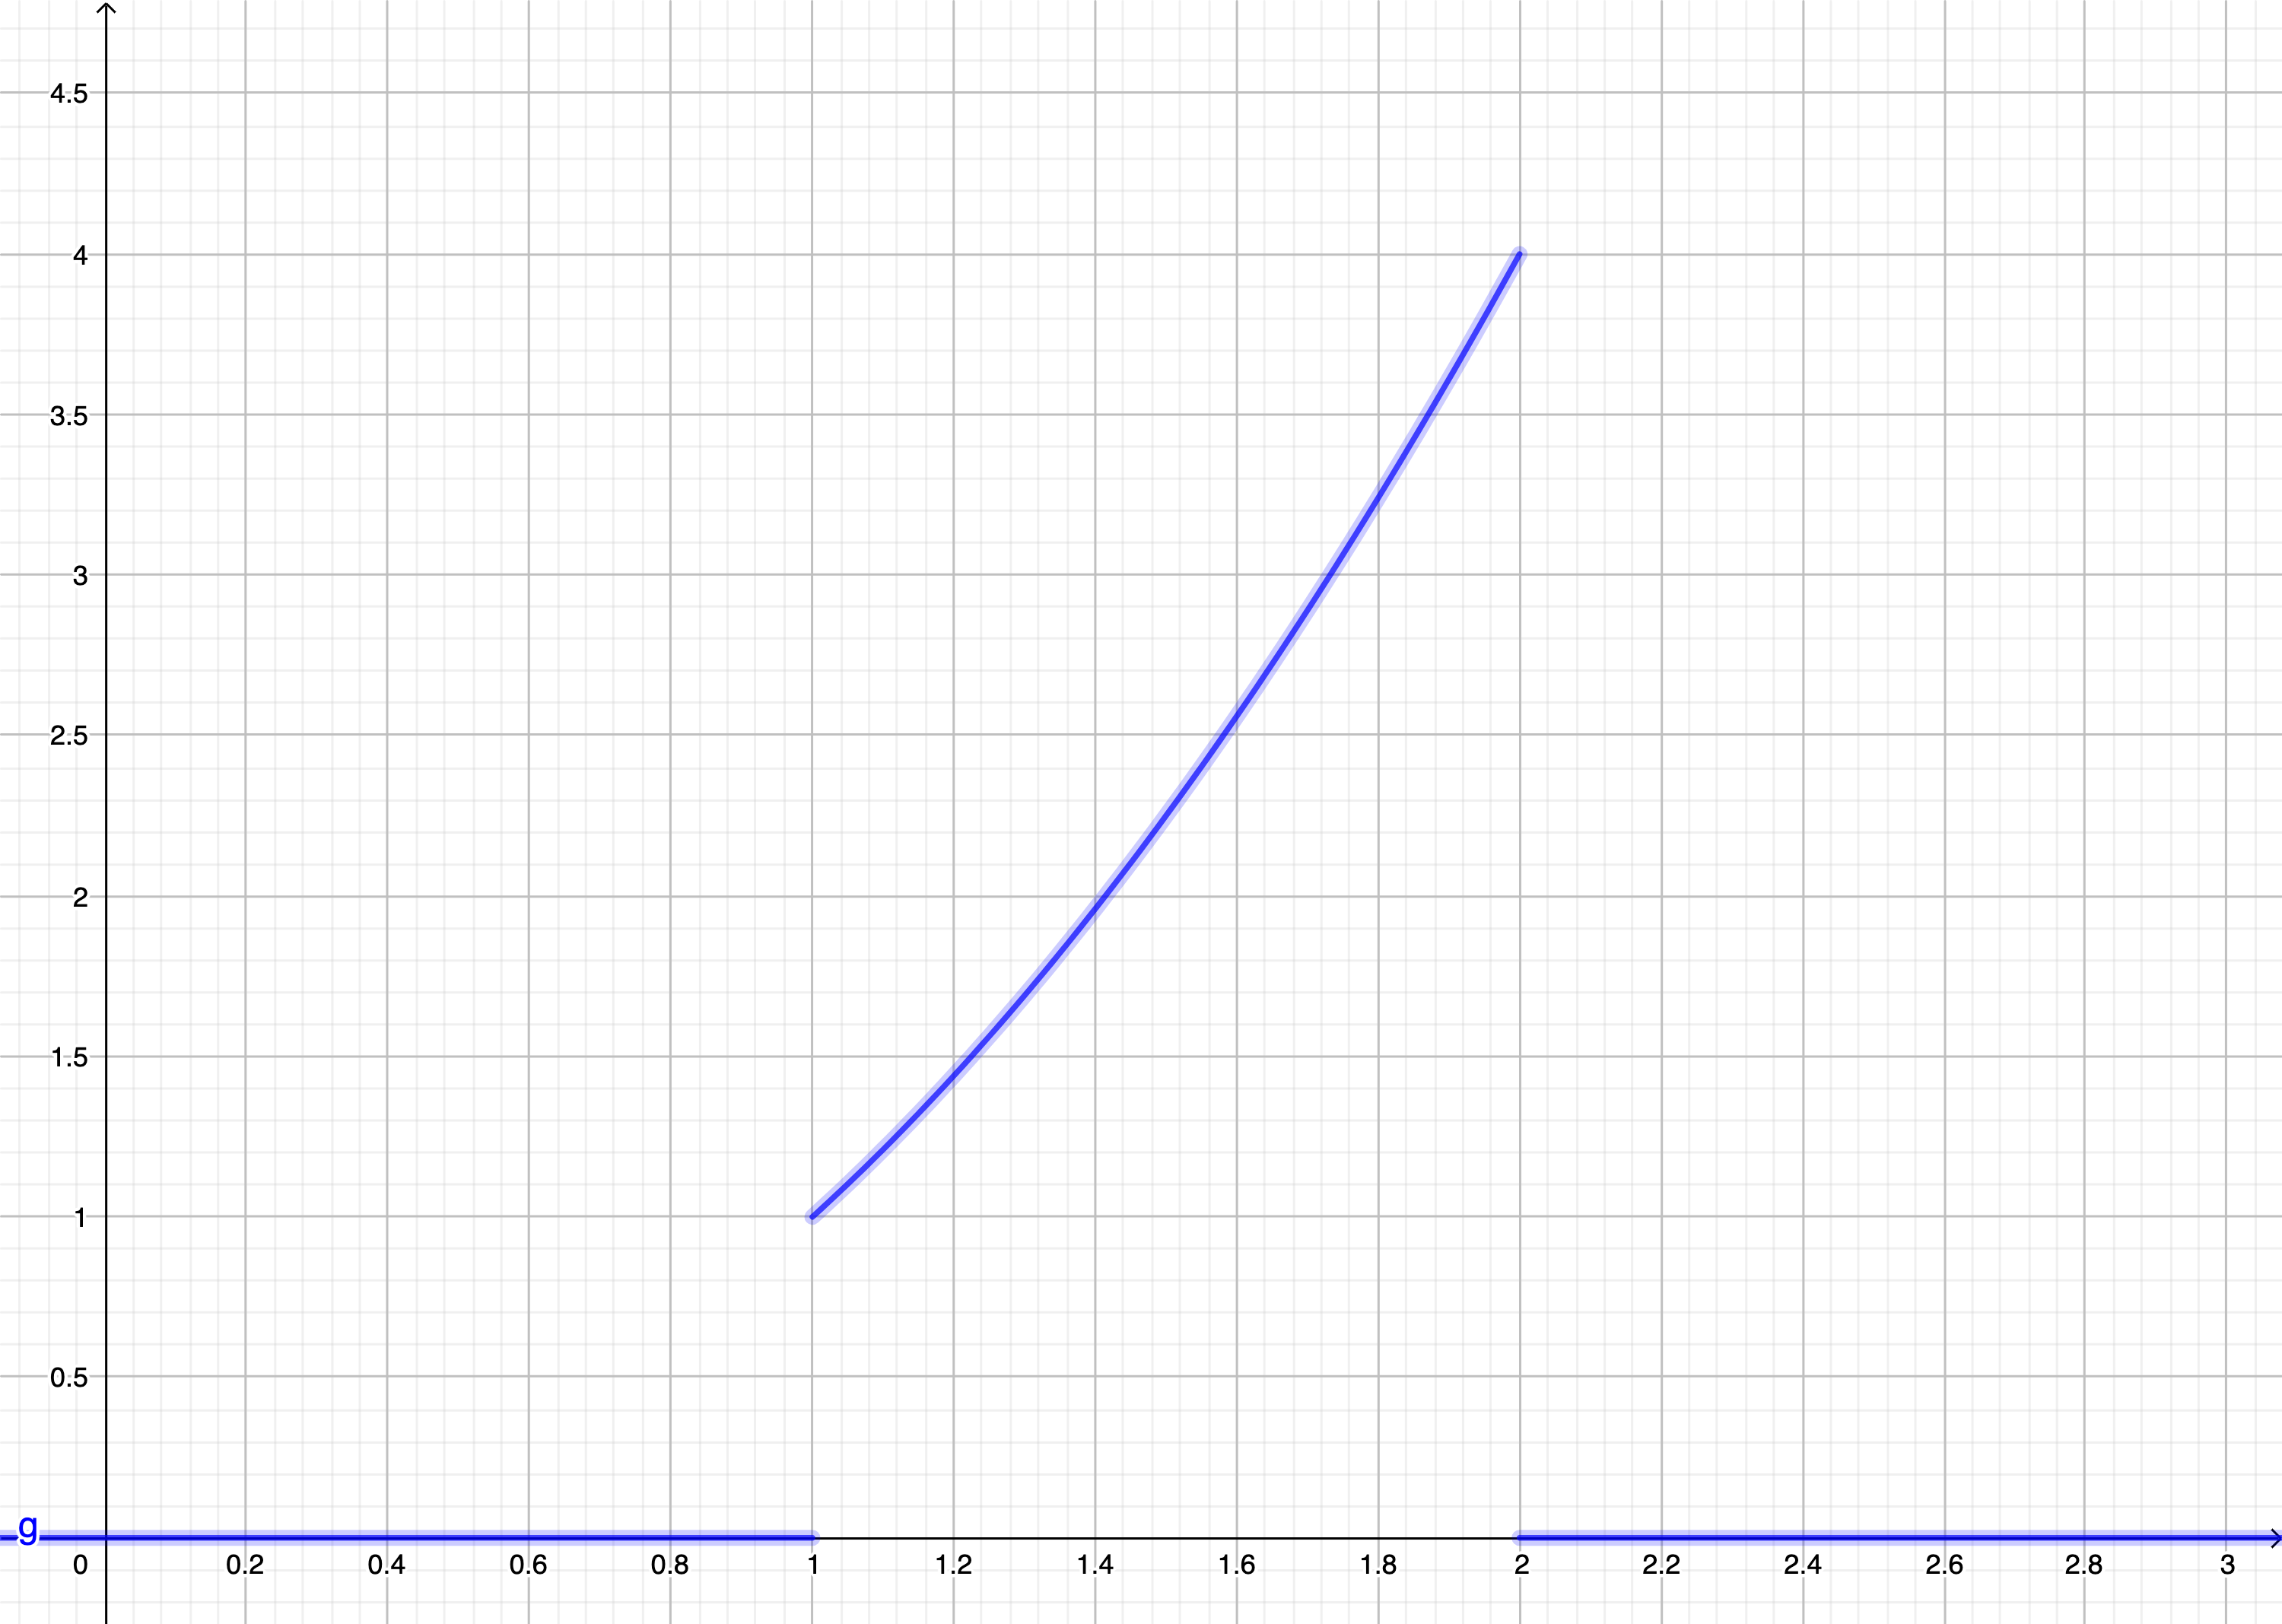
\includegraphics[scale=3]{../figure_6_3_8.png}
	\caption{Plot of $f(t)$.}
\end{figure}
\begin{align*}
	\Laplace\{f\}
	&= \Laplace\{t^2[u(t-1) - u(t-2)]\} \\
	&= \Laplace\{[(t-1)^2+2(t-1)+1]u(t-1)\} - \Laplace\{[(t-2)^2 + 4(t-2) + 4]u(t-1)\} \\
	&= \Laplace\{(t-1)^2u(t-1)\}
		+ 2 \Laplace\{(t-1)u(t-1)\}
		+ \Laplace\{u(t-1)\} \\
	&\hspace*{1cm} - (\Laplace\{(t-2)^2u(t-2)\}
	+ 4 \Laplace\{(t-2)u(t-2)\}
	+ 4 \Laplace\{u(t-2)\}
	) \\
	&= \frac{e^{-s}}{s^3} (s^2+2s+2) - \frac{2e^{-2s}}{s^3} (2s^2+2s+1)
\end{align*}

\section*{6.3.15}
\begin{align*}
	F(s) 
	&= \frac{e^{-2s}}{s^6} 
	= e^{-2s} \cdot \frac{5!}{s^{5+1}} \cdot \frac{1}{5!} \\
	\rightarrow \Laplace^{-1}\{F\}
	&= u(t-2) \cdot (t-2)^5 \cdot \frac{1}{120}
	= \frac{(t-2)^5 u(t-2)}{120}
	\hspace*{.7cm} \text{(from table.)}
\end{align*}

\newpage
\section*{6.3.25}
We are solving the IVP
\begin{align*}
	\left\{\begin{matrix}
	y'' + y = 2t & 0 \leq t < 1 \\ 
	2 & t > 1 
	\end{matrix}\right.
\end{align*}
with $y(0) = 0,\ y'(0) = -2$.
\begin{itemize}[leftmargin=4.0cm,labelsep=0.5cm]
\item[$\Laplace$ - transform:]
	$\Laplace\{y'' + y\} = \Laplace\{2t\} 
	\rightarrow s^2Y + 2 + Y = \frac{2}{s^2}$
\item[Solve for $Y$:]
	$Y = \frac{2}{s^2(s^2+1)} - \frac{2}{s^2+1}$
\item[Write as partial fraction:]
	$2 = As^3 + (B+C)s^2 + As + B \\
	\rightarrow A = 0,\ B = 2,\ C = -2 \\
	\rightarrow Y = \frac{2}{s^2} - \frac{4}{s^2+1}$
\item[Inverse $\Laplace$ -transform:]
	$y = \Laplace^{-1}\{Y\}
	= \Laplace^{-1}\left\{\frac{2}{s^2}\right\} - \Laplace^{-1}\left\{\frac{4}{s^2+1}\right\} \\
	y = 2t - 4\sin t$
\item[Control:]
	$y(0) = 0 - 0 = 0 \\
	y' = 2 - 4 \cos t \\
	\rightarrow y'(0) = 2 - 4 = -2 \\
	y'' = 4 \sin t \\
	\rightarrow y'' + y = 4 \sin t + 2t - 4 \sin t = 2t
	\hspace*{0.5cm} \text{Ok.}$
\end{itemize}
Hence,
\begin{align*}
	y(t) = 
	\left\{\begin{matrix}
	2t - 4 \sin t & 0 < t < 1 \\ 
	2 & t > 1.
	\end{matrix}\right.
\end{align*}

\end{document}
